\section{Theory of Operation}
\label{sec:theory}

HCCP has roots in LEACH, following the design of clusterhead elections, but extends the design of LEACH 
in multiple ways. While LEACH has relatively simple clusterhead elections, where nodes
elect themselves based on a probability, HCCP has a more elaborate election process. HCCP's election 
process weighs the `goodness' of the node to be a clusterhead, and automatically limits the number of other nodes that 
will be clusterheads. HCCP has also adopted the way a LEACH network cycles between clusterhead
elections and node runtime.

The LEACH run cycle is quite simple in it's operation, and provided inspiration for the HCCP
run cycle. The LEACH network cycle is as follows:

\begin{figure}[htbp]
	\centering
		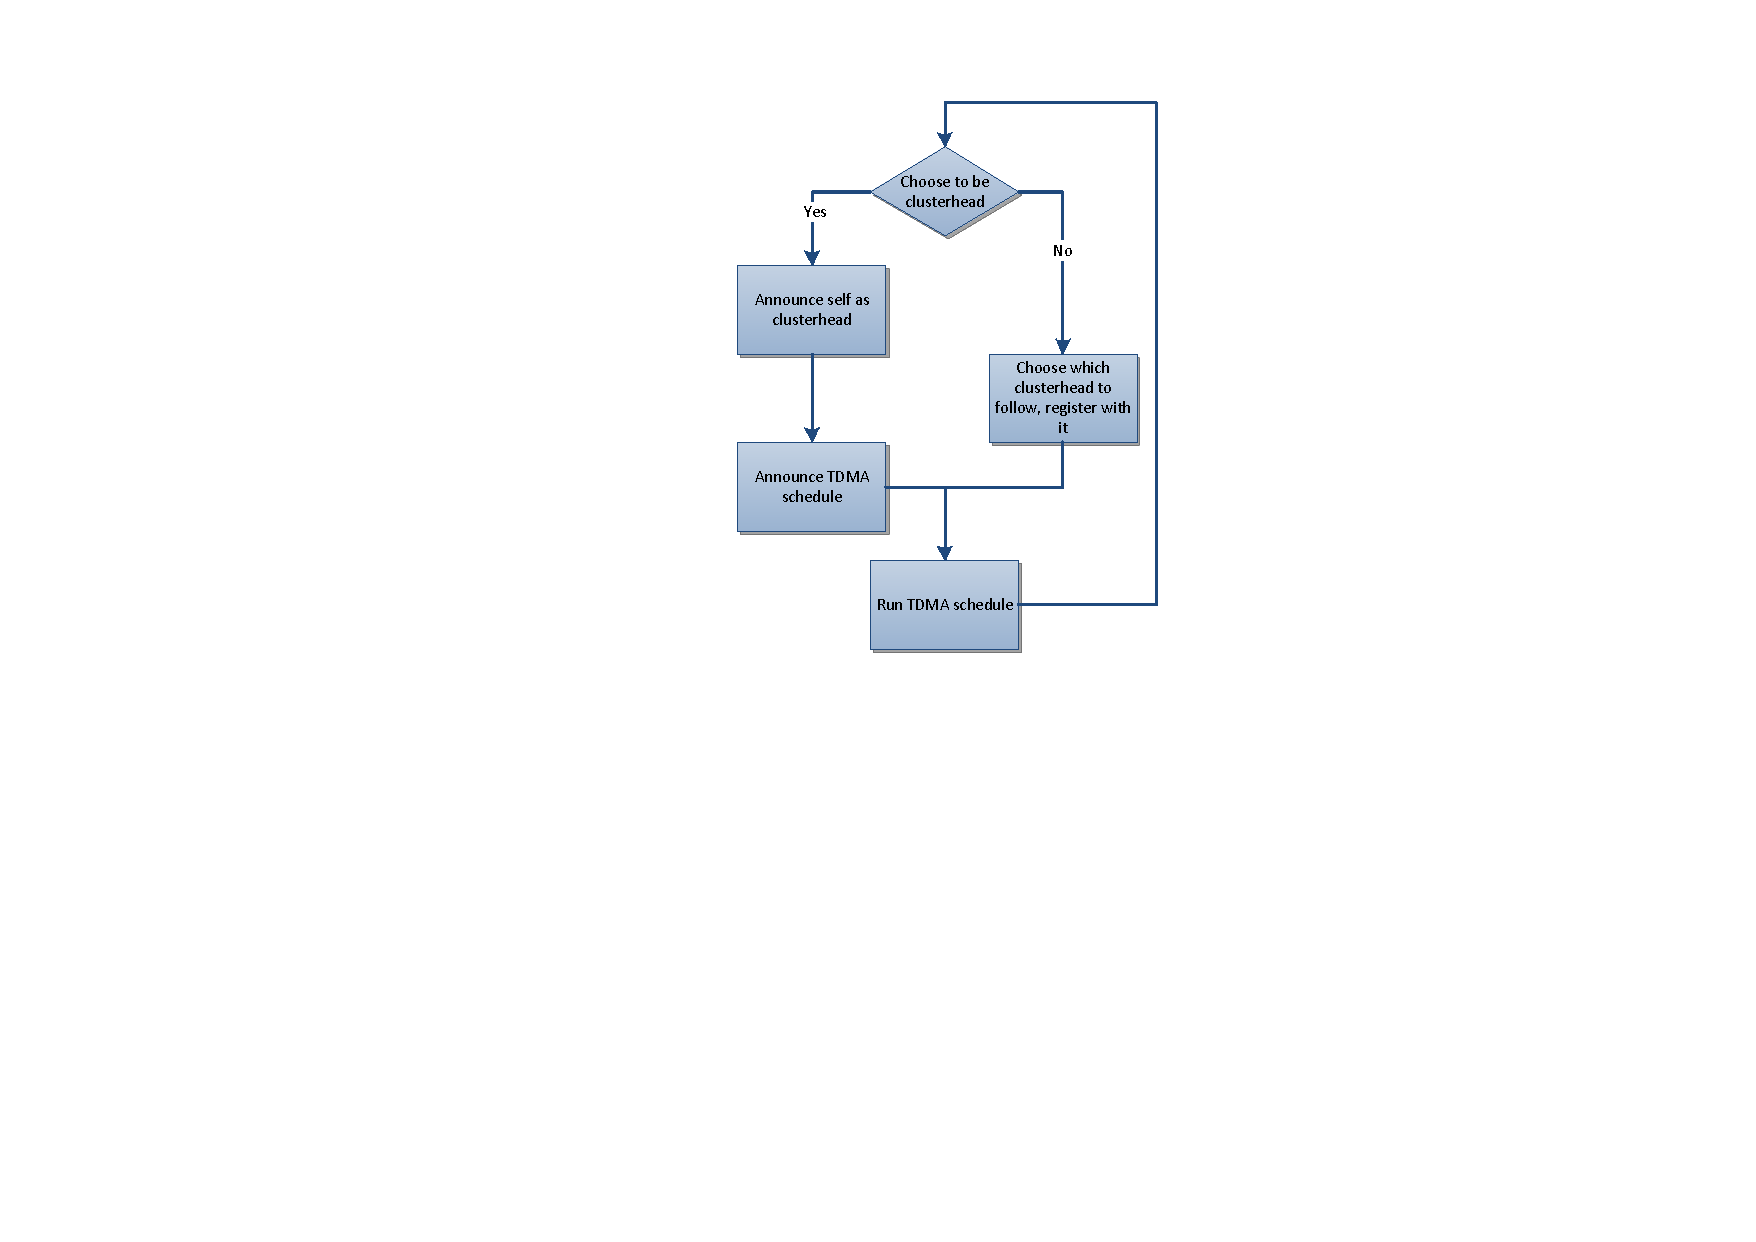
\includegraphics[height=4.2in]{images/protocol/LeachFlowchart.pdf}
	\caption{LEACH election run cycle.}
	\label{fig:leachelec}
\end{figure}

\begin{enumerate}
	\item \textbf{Clusterhead election} --- Motes choose whether not not to advertise themselves as
	clusterheads. The decision to be clusterhead is based on a how long it has been since it was a 
	clusterhead and some added randomness.
	\item \textbf{Choose cluster} --- Motes that are not clusterheads send messages to the
	clusterhead they will follow this round.
	\item \textbf{Announce Schedule} --- Clusterhead sends a TDMA % TDMA defined eariler
	schedule via broadcast. 
	\item \textbf{Cluster Runtime} --- The motes in the cluster follow the TDMA schedule, 
	taking turns sending messages to the clusterhead.
	\item \textbf{Repeat} --- Go back to clusterhead election. There can be a sleep time here to extend the network life.
\end{enumerate}


THE LEACH network cycle can be seen graphically on Figure~\ref{fig:leachelec}. The cycle is repeated until all the 
motes in the network cease to function. LEACH was focused 
on simplicity, which makes LEACH quite robust as it runs. Since every mote takes becomes a clusterhead
occasionally, there is no single point of failure -- the network will continue to function even
if a number of motes cease to function. LEACH makes a solid foundation to build upon, using the 
lessons learned from its success and building on its weaknesses.


HCCP takes the strengths LEACH, using the simplicity of the election and run cycles, adding
the ability to leverage the heterogeneity that is inherent in all WSNs. The HCCP network cycle 
is as follows and is illustrated  in Figure~\ref{fig:images_protocol_ElectionFlowchart}.


\begin{enumerate}
	\item \textbf{Clusterhead Election}
	\begin{enumerate}
		\item \textbf{Announce Candidacy} --- Announce the mote's intentions to be clusterhead. 
		Using a Goodness assessment, announce first if the mote has a good assessment.
		\item \textbf{Announce Clusterhead} - Successful candidates announce they are clusterheads.
	\end{enumerate}
	\item \textbf{Choose Cluster} --- Same as LEACH.
	\item \textbf{Announce Schedule} --- Same as LEACH. 
	\item \textbf{Cluster Runtime} --- Same as LEACH.
	\item \textbf{Roundtable Discussion} --- Any queries or announcements can be made at this time. 
	Clusterheads can opt-out, forcing a clusterhead election.
	\item \textbf{Repeat} --- Go back to Cluster Runtime for multiple iterations. Every $n^{th}$ iteration 
	(where $n$ is selected before network deployment and well-known to the network) go back to Clusterhead election.
	
\end{enumerate}

\begin{figure}[ht]
	\centering
		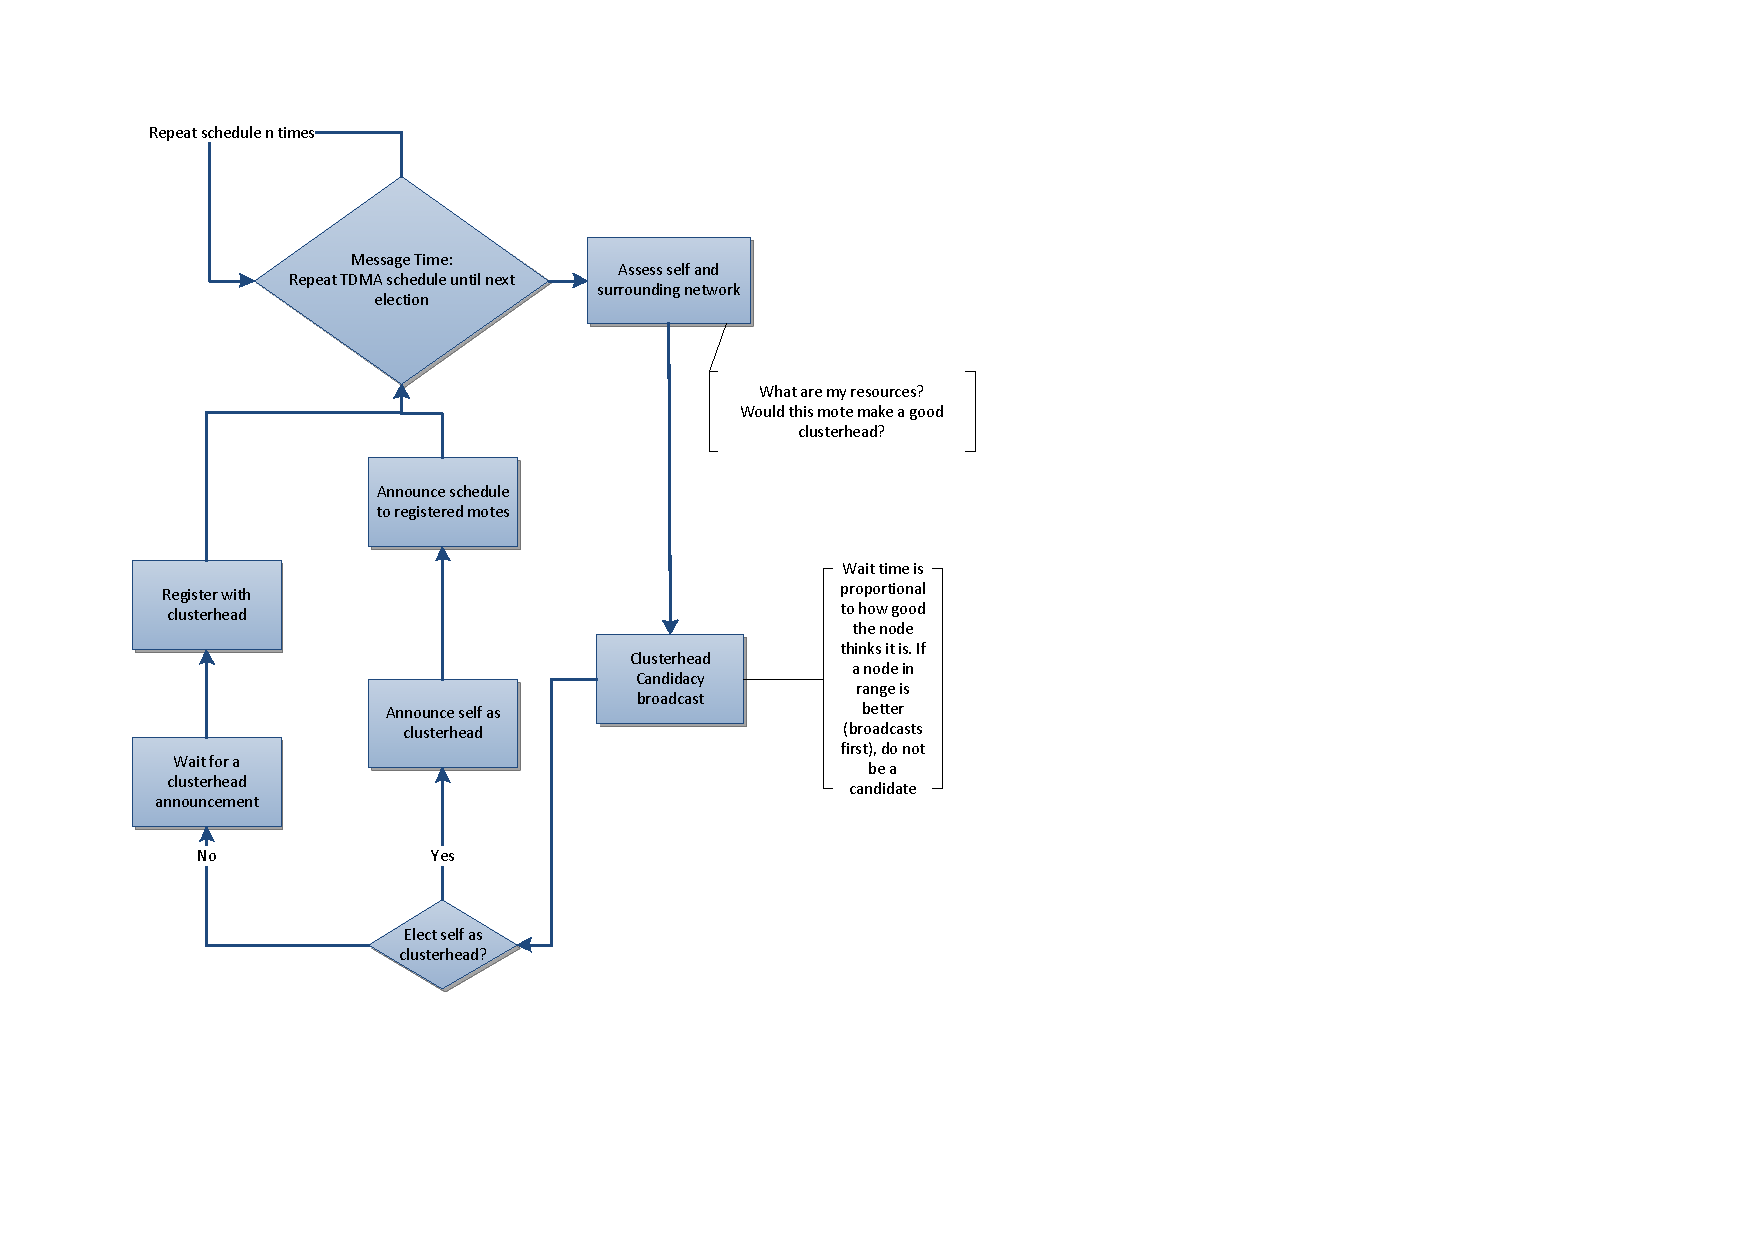
\includegraphics[height=5.75in]{images/protocol/ElectionFlowchart.pdf}
	\caption{A visualization of the HCCP election and run cycle.}
	\label{fig:images_protocol_ElectionFlowchart}
\end{figure}

HCCP uses all of the strengths of LEACH in the run cycle, further modifying the 
concept with some extra modifications that make
the network more intelligent in terms of which motes are elected clusterhead. The major additions are two-stage elections,
multiple iterations of the TDMA schedule and Roundtable Discussion (including Clusterhead opt-outs).

\subsubsection* {Two-stage election}
	Motes choose to be a clusterhead candidate before they can elect themselves clusterheads. 
	A mote determines that it would be a good clusterhead by inspecting its available resources,
	and choosing how long to wait before they announce themselves as a clusterhead.
	Motes that announce candidacy first get to be clusterheads that round.
	Motes that determine they would not be 
	very good clusterheads wait a longer time due to the Goodness Delay. If a candidacy announcement 
	from a better potential clusterhead that is relatively close in proximity 
	is overheard before a candidate broadcasts, the lesser candidate will
	not send an announcement, and demote itself to a regular cluster member.
	
\subsubsection* {Multiple iterations of schedule}
	All messages in clusterhead elections can be considered overhead, as these messages are not
	relaying any information to any destination. Further, 
	any time a mote is on without sending or receiving messages
	can also be considered overhead.
	
	To minimize time spent in clusterhead elections, they should only be run
	occasionally. LEACH runs a clusterhead election after every TDMA schedule runtime,
	which is good for distributing the burden of being a clusterhead, but creates
	lots of overhead messages. 
	
	The solution to this is relatively simple; a clusterhead election should only happen 
	occasionally. Further, a TDMA schedule does not need to be re-transmitted before
	every TDMA runtime. A TDMA schedule only needs to be transmitted after a 
	clusterhead election, which should only happen after $n$ runs of 
	the TDMA schedule. The number of times the network TDMA schedule executes ($n$) should be determined before
	network deployment. This is so it is well-known, consistent number across the entire network
	ensuring that the network does not get out of synchronization. A lower
	value of $n$ should be chosen if the network is to be adaptive and flexible, while
	a larger value of $n$ should be chosen if the network should have as little overhead as possible.

\subsubsection* {Roundtable Discussion}
	After each run of the TDMA schedule, all the motes in the network turn on 
	their radios to listen for broadcasted announcements or queries.
	This is the time where clusterheads can opt-out, synchronization messages
	can be exchanged and routing tables can be shared. The Roundtable Discussion 
	time can also be used to extend HCCP in various ways, providing a
	time to implement neighbour discovery and adjust radio power accordingly, or whatever
	the network administrator chooses.



\subsubsection* {Clusterhead opt-out}
\label{optout}
	Since the TDMA schedule published by the clusterhead will be followed 
	multiple times, the clusterhead's performance may degrade, eventually causing
	the entire cluster to perform poorly. LEACH averts this problem by running 
	a clusterhead election after every TDMA schedule runtime.
	Since HCCP runs multiple iterations of the TDMA schedule, the clusterhead needs a
	way to retire if it begins to degrade.

	A clusterhead can announce its retirement during the Roundtable Discussion. 
	When a clusterhead retires,
	it forces a small clusterhead election, with only the motes in the 
	one affected cluster acting in the clusterhead election. The network
	does a LEACH-style clusterhead election. The first mote that announces
	that it is a clusterhead becomes the new clusterhead for the cluster.
	The Goodness Delay is used to decide how long a mote will wait before
	it sends a clusterhead announcement, using the same method as candidacy announcements.
	This way, the best possible clusterhead mote should become the replacement clusterhead.


	The cluster then continues to run using the existing TDMA schedule
	for the remaining  iterations
	before the next full clusterhead election.



